\section{Discusión}
El código de este trabajo utiliza las funciones en lenguaje \code{C} del trabajo anterior 
y nuevas funciones en assembler. El trabajo en assembler está separado en un 
archivo por filtro a aplicar y un archivo para las \keyword{macros} en común, utilizadas 
por los filtros.
		
A continuación se detallara lo escrito y pensado para los diferentes algoritmos,
que fueron ajustados para mejor rendimiento según la matríz utilizada. Antes de 
empezar se definen nombres específicos (\keyword{macros}) para cada registro \code{xmm}, para facilitar la 
lectura del código. Los nombres definidos son: \code{srcl}, \code{srch} que contendrán las 
líneas leídas de la imagen original; \code{acul}, \code{acuh} que acumularán los resultados 
parciales del cálculo; y cuatro registros temporales \code{tmp1}, \code{tmp2}, \code{tmp3} y \code{tmp4} 
(en el caso del \keyword{Frei-Chen} el cuarto registro temporal se renombra a \code{sqrt2}).

Los algoritmos siguen una línea general, empiezan y terminan con lo definido en la convención C, 
se definen nombres de variables para los parámetros y se usan los registros generales de la siguiente manera:
\vspace{5mm}

\begin{tabular}{l p{10cm}}
	\code{eax}:&Almacena las variables \code{xOrder} e \code{yOrder} que indican sobre qué derivada realizar el procesamiento. \\
	\code{ebx}:&Contador para las filas. \\
	\code{ecx}:&Contador para las columnas. \\
	\code{edx}:&Ancho de la imagen. \\
	\code{esi}:&Puntero a la imagen fuente. \\
	\code{edi}:&Puntero a la imagen destino.
\end{tabular}

\vspace{5mm}
	Luego para cada fila de la imagen se realiza el procesamiento sobre la derivada de \code{x} o de \code{y} según sea necesario 
procesando de a 14 píxeles, y antes de terminar la fila se revisa si se pueden calcular exactamente 14 píxeles, sino se retroceden los 
punteros para poder lograrlo y se pasa a la siguiente fila.

\vspace{1cm}

\subsection{Estructura básica para \keyword{Sobel}, \keyword{Prewitt} y \keyword{Frei-Chen}}
	Los algoritmos de \keyword{Sobel}, \keyword{Prewitt} y \keyword{Frei-Chen} están estructurados de la misma manera. Cada uno tiene 
definidas sus propias \keyword{macros} denominadas \code{procesarLineaX}, \code{procesarLineaY}, \code{calcularX} y \code{calcularY}. 
De esta manera, el código de los tres filtros es bastante similar y para comprenderlos basta con entender la estructura básica de uno de 
ellos y luego los detalles particulares. La idea general del procesamiento se basa en las \keyword{macros} \code{procesarLineaX/Y}. Cada 
\keyword{macro} se encarga de leer 16 píxeles, desempaquetarlos, hacer el procesamiento de los 14 píxeles procesables según la línea correspondiente de la 
matríz, y sumar el resultado de la operación en dos acumuladores. Las macros \code{calcularX} y \code{calcularY} son las encargadas de 
efectuar el procesamiento en paralelo de 6 píxeles convertidos a \keyword{word}. Cada algoritmo tiene sus versiones de ambas \keyword{macros}.
 Como estas \keyword{macros} no procesan todos los píxeles necesarios por limitaciones del método, cada algoritmo calcula individualmente 
los 2 píxeles centrales de los 16 levantados. Por último, se empaquetan los datos a \keyword{bytes}, se guardan en la imagen resultante y
se avanza en la imagen hasta completar el procesamiento. A continuación serán explicados los diferentes algoritmos de paralelización utilizados 
en cada caso.

\subsection{Sobel}

\subsubsection{Procesamiento en \code{x}}
	La \keyword{macro} \code{procesarLineaX} comienza cargando en los registros \code{srcl} y \code{srch} 16 píxeles de la imagen original, 
luego desempaqueta a ocho \keyword{words} adecuadamente con las instrucciones \code{punpcklbw} (\keyword{Unpack Low Bytes to Words}) y \code{punpckhbw} 
(\keyword{Unpack High Bytes to Words}). Mediante la \keyword{macro} \code{calcularX} se trabajan ocho píxeles, que serán primero los menos significativos 
(contienidos en el registro \code{srcl}) y después los más significativos (contenidos en el registro \code{srch}). Al aplicar convolución entre la primer 
línea de la matríz de \keyword{Sobel} ( 
\code{
\begin{tabular}{|c|c|c|}
	\hline
	-1 & 0 & 1 \\
	\hline
\end{tabular} 
}
) y una línea genérica 
\code{
\begin{tabular}{|c|c|c|c}
	\hline
	a & b & c & ... \\
	\hline
\end{tabular}
}
, el resultado esperado es 
\code{
\begin{tabular}{|c|c|c|}
	\hline
	c-a & d-b & e-c \\
	\hline
\end{tabular}
}.
La \keyword{macro} \code{calcularX} obtiene el resultado esperado de 6 píxeles en paralelo para \keyword{Sobel} en \code{x} de la siguiente manera:

\begin{center}
\code{
\begin{tabular}{r c l}
	src	&\reg{a}{b}{c}{d}{e}{f}{g}{h} &	\keyword{parámetro}	\\ \\
	tmp1	&\reg{a}{b}{c}{d}{e}{f}{g}{h} &	\keyword{copia src a tmp1}		\\ \\
	tmp1	&\reg{c}{d}{e}{f}{g}{h}{0}{0} & \keyword{shift 2 words $\leftarrow$}	\\ \\
	tmp1	&{\tiny\reg{c-a}{d-b}{e-c}{f-d}{g-e}{h-f}{-g}{-h}} & \keyword{resta src a tmp1} \\ \\
%	tmp1	&{\tiny\reg{000}{000}{c-a}{d-b}{e-c}{f-d}{g-e}{h-f}} & \keyword{shift 2 words $\rightarrow$} \\ \\
%	tmp1	&{\tiny\reg{000}{c-a}{d-b}{e-c}{f-d}{g-e}{h-f}{000}} & \keyword{shift 1 word $\leftarrow$} \\ \\
\end{tabular}
}
\end{center}

Luego de obtener el resultado mostrado en el esquema, se suman los 6 resultados válidos al acumulador correspondiente. 
Como la primer y tercer líneas de la matríz de \keyword{Sobel} son iguales y la segunda es el doble de la primera, se procesan todas las líneas 
con la misma \keyword{macro}. En el caso de estar procesando la segunda línea de la matríz (
\code{
\begin{tabular}{|c|c|c|}
	\hline
	-2 & 0 & 2 \\
	\hline
\end{tabular} 
}
), después de ejecutar la \keyword{macro} \code{calcularX}, se duplica el resultado obtenido.

	Los valores intermedios se acumulan en \code{acul} y \code{acuh}. Una vez calculados, se procesan individualmente y aprovechando los resultados
intermedios obtenidos, los dos píxeles centrales de los 14 píxeles originales que debían ser procesados ya que este método impide procesarlos en paralelo.

\subsubsection{Procesamiento en \code{y}}
	La idea detrás del procesamiento de Sobel en \code{y} es básicamente la misma al procesamiento en \code{x}. En este caso, al aplicar convolución 
entre la primer línea de la matríz (
\code{
\begin{tabular}{|c|c|c|}
	\hline
	-1 & -2 & -1 \\
	\hline
\end{tabular} 
}
) y una línea genérica (
\code{
\begin{tabular}{|c|c|c|c}
	\hline
	a & b & c & ... \\
	\hline
\end{tabular} 
}
), el resultado esperado es 
\code{
\begin{tabular}{|c|c|c|}
	\hline
	-a-2b-c & -b-2c-d & -c-2d-e \\
	\hline
\end{tabular}
}. Para obtener este resultado, se realiza el siguiente procedimiento:
\begin{center}
\code{
\begin{tabular}{c r c l}
	&src	&\reg{a}{b}{c}{d}{e}{f}{g}{h} &	\keyword{parámetro}	\\ \\
	(1)&tmp1	&\reg{a}{b}{c}{d}{e}{f}{g}{h} &	\keyword{copia src a tmp1}		\\ \\
	(2)&tmp1	&\reg{b}{c}{d}{e}{f}{g}{h}{0} &	\keyword{shift 1 word $\leftarrow$}	\\ \\
	(3)&tmp1	&\reg{2b}{2c}{2d}{2e}{2f}{2g}{2h}{0} &	\keyword{duplica tmp1}		\\ \\
	(4)&tmp1	&\tiny\reg{a+2b}{b+2c}{c+2d}{d+2e}{e+2f}{f+2g}{g+2h}{h} & \keyword{suma src a tmp1} \\ \\
	(5)&tmp2	&\reg{a}{b}{c}{d}{e}{f}{g}{h} &	\keyword{copia src a tmp2}		\\ \\
	(6)&tmp2	&\reg{c}{d}{e}{f}{g}{h}{0}{0} & \keyword{shift 2 words $\leftarrow$}	\\ \\
	(7)&tmp1	&\tiny\reg{a+2b+c}{b+2c+d}{c+2d+e}{d+2e+f}{e+2f+g}{f+2g+h}{g+2h}{h} & \keyword{suma tmp2 a tmp1} \\ \\
\end{tabular}
}
\end{center}

Luego de obtener el resultado mostrado en el esquema, se acumula el resultado de \code{calcularY} restando (en caso de estar calculando la primer 
línea de la matríz) o sumando (si se trata de la tercera). Esto se debe a que la matríz es igual en ambas líneas, salvo porque la primer línea es 
negativa. Como la matríz contiene sólo ceros en la segunda línea, no es necesario realizar los cálculos.

Al igual que para \keyword{Sobel} en \code{x}, después de calcular los resultados intermedios, se procesan individualmente los 2 píxeles faltantes.

\begin{center}
\includegraphics[scale=0.5]{../imgs/steam-engine.jpg}
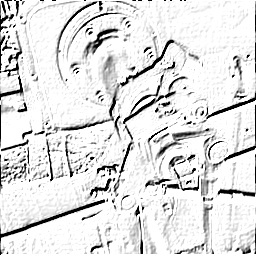
\includegraphics[scale=0.5]{../imgs/steam-engine-sobel.jpg}\\
\texttt{\small Ejemplo del filtro Sobel negado}\\
\end{center}


\vspace{5mm}
\subsection{Prewitt}
	Este algoritmo es casi idéntico al anterior. El único cambio general es que, luego de procesar las líneas pero antes
de empaquetar a \keyword{bytes}, se calcula el valor absoluto de los acumuladores.
\subsubsection{Procesamiento en \code{x}}
	El cálculo de \keyword{Prewitt} en \code{x} es idéntico al de la primer línea de \keyword{Sobel}. Basta con no cambiar de línea y realizar
los mismos pasos para obtener el resultado correcto.

\subsubsection{Procesamiento en \code{y}}
	El cálculo de \keyword{Prewitt} en \code{y} es similar al de \keyword{Sobel}. El único cambio en el algoritmo es que no se efectúa el paso (3). 
es decir, no se duplica el valor de la segunda columna de \code{src} sino que se suma directamente.

\begin{center}
\vspace{1.0cm}
\includegraphics[scale=0.5]{imgs/steam-engine.jpg}
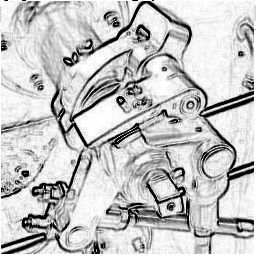
\includegraphics[scale=0.5]{imgs/steam-engine-prewitt-neg.jpg} \\*
\texttt{\small Ejemplo del filtro Prewitt negado } \\
\end{center}

\vspace{5mm}
\subsection{Frei-Chen}
	La matríz de \keyword{Frei-Chen} contiene números reales además de números enteros. Para hacer de forma más eficiente el algoritmo, 
primero se precalcula $\sqrt{2}$ en un registro temporal (\code{sqrt2}) mediante la instrucción \code{sqrtps} (\keyword{Square Root Parallel 
Single}) ya que es el único número real presente en la matríz.

\vspace{5mm}
\begin{center}
\code{
\begin{tabular}{r c l}
	sqrt2	&\sreg{$\sqrt{2}$}{$\sqrt{2}$}{$\sqrt{2}$}{$\sqrt{2}$}&	\keyword{raíces de 2}	\\ \\
\end{tabular}
}
\end{center}

Al tener que multiplicar por un número real, los cálculos intermedios son convertidos a \keyword{float}. Por limitaciones del set de instrucciones
\code{IA-32}, a la hora de realizar la conversión, se extienden los enteros de 16 \keyword{bits} a 32 \keyword{bits}. Para realizar la extensión signada,
se utilizó la instrucción \code{pcmpgtw} junto con \code{punpckhwd} y \code{punpcklwd} comparando el registro a extender con un registro en 0 como se 
muestra en el siguiente ejemplo:
\begin{center}
\code{
\begin{tabular}{r c l}
	tmp3	&\reg{0}{0}{0}{0}{0}{0}{0}{0}& \keyword{tmp3 = 0} \\ \\
	tmp1	&{\tiny\reg{-5}{123}{-145}{100}{66}{-93}{80}{3}} & \keyword{tmp1 en words} \\ \\
	tmp2	&{\tiny\reg{-5}{123}{-145}{100}{66}{-93}{80}{3}} & \keyword{tmp2 = tmp1} \\ \\
	tmp3	&{\tiny\reg{0xFFFF}{0}{0xFFFF}{0}{0}{0xFFFF}{0}{0}} & pcmpgtw \keyword{tmp2, tmp3} \\ \\
	tmp1	&\sreg{-5}{123}{-145}{100}& punpcklwd \keyword{tmp1, tmp3} \\ \\
	tmp2	&\sreg{66}{-93}{80}{3}& punpckhwd \keyword{tmp2, tmp3} \\ \\
\end{tabular}
}
\end{center}
Al igual que en \keyword{Prewitt}, luego de procesar las líneas pero antes de empaquetar a \keyword{bytes}, se calcula el valor absoluto de 
los acumuladores.

\subsubsection{Procesamiento en \code{x}}
	El algoritmo realizado para \keyword{Frei-Chen} en \code{x} es similar al de \keyword{Sobel}. En este caso, la diferencia reside 
únicamente en el cálculo de la segunda línea de la matríz (
\code{
\begin{tabular}{|c|c|c|}
	\hline
	$-\sqrt{2}$ & 0 & $\sqrt{2}$ \\
	\hline
\end{tabular} 
}
). Para calcular esta línea, se aprovecha la propiedad distributiva de la multiplicación respecto de la suma y la resta, calculando primero la resta 
en enteros, luego convirtiendo a \keyword{float} y multiplicando el resultado por $\sqrt{2}$. Una vez hechas las operaciones, se convierte el resultado 
de \keyword{float} a \keyword{dword}, para finalmente convertirlo a \keyword{word}.

\begin{center}
\code{\small
\begin{tabular}{r c l}
	src	&\reg{a}{b}{c}{d}{e}{f}{g}{h} &	\keyword{parámetro}	\\ \\
	tmp1	&{\tiny\reg{c-a}{d-b}{e-c}{f-d}{g-e}{h-f}{-g}{-h}} & \keyword{resta src a tmp1} \\ \\
	tmp2	&\sreg{g-e}{h-f}{-g}{-h} & \keyword{tmp2 = (float)tmp1[4..7]} \\ \\
	tmp1	&\sreg{c-a}{d-b}{e-c}{f-d} & \keyword{tmp1 = (float)tmp1[0..3]} \\ \\
	tmp1	&\sreg{(c-a)$\sqrt{2}$}{(d-b)$\sqrt{2}$}{(e-c)$\sqrt{2}$}{(f-d)$\sqrt{2}$} & \keyword{tmp1 = (dword) (tmp1 * sqrt2) } \\ \\
	tmp2	&\sreg{(g-e)$\sqrt{2}$}{(h-f)$\sqrt{2}$}{(-g)$\sqrt{2}$}{(-h)$\sqrt{2}$} & \keyword{tmp2 = (dword) (tmp2 * sqrt2) } \\ \\
	tmp1	&{\tiny\reg{(c-a)$\sqrt{2}$}{(d-b)$\sqrt{2}$}{(e-c)$\sqrt{2}$}{(f-d)$\sqrt{2}$}{(g-e)$\sqrt{2}$}{(h-f)$\sqrt{2}$}{(-g)$\sqrt{2}$}{(-h)$\sqrt{2}$}} & \keyword{tmp1 = (word)tmp1, (word)tmp2 } \\ \\
	\end{tabular}
}
\end{center}

Luego el algoritmo continúa igual que el algoritmo de \keyword{Sobel}, salvando los cálculos individuales de los píxeles centrales que vuelve a realizar 
un procedimiento similar al ya mostrado.


\subsubsection{Procesamiento en \code{y}}
	Siguiendo la idea de la implementación de \keyword{Sobel}, el algoritmo para \keyword{Frei-Chen} en \code{y}, se diferencia en la segunda 
columna de la matríz, que está multiplicada por $\sqrt{2}$ en lugar de por 2. La única diferencia con \keyword{Sobel} se va a encontrar en que se 
necesita realizar la multiplicación en punto flotante en cada llamada a la macro \code{calcularY}. Es decir, se reemplaza el paso (3) del algoritmo
de \keyword{Sobel} por la conversión a punto flotante y la multiplicación por $\sqrt{2}$. La forma de multiplicar es igual a la utilizada para
\keyword{Frei-Chen} en \code{x} y descripta anteriormente.

\begin{center}
\vspace{1.0cm}
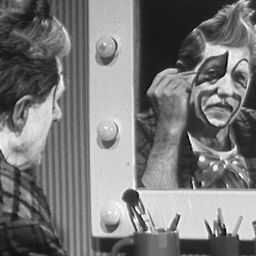
\includegraphics[scale=0.5]{../imgs/cln1.jpg}
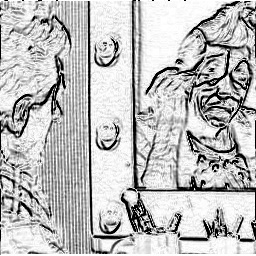
\includegraphics[scale=0.5]{../imgs/cln1-frei-chen.jpg} \\*
\texttt{\small Ejemplo del filtro Frei-Chen negado } \\
\end{center}

\subsection{Roberts}
La implementación del operador de \keyword{Roberts}, se basa en la explicada anteriormente para \keyword{Sobel}, pero es más simple y concisa, 
ya que la matríz es de 2x2. La principal ventaja de este tamaño de matríz es que permite calcular de a 15 píxeles. Al igual que en el algoritmo 
de \keyword{Prewitt} y \keyword{Frei-Chen}, luego de procesar las líneas pero antes de empaquetar a \keyword{bytes}, se calcula el valor absoluto 
de los acumuladores.

\subsubsection{Procesamiento en \code{x}}	
	La macro \code{RobertsX} obtiene 16 píxeles, los desempaqueta a \keyword{words} y los suma a los acumuladores directamente, ya que la
primer línea de la matríz de \keyword{Roberts} es 
\code{
\begin{tabular}{|c|c|}
	\hline
	1 & 0 \\
	\hline
\end{tabular} 
}. Luego avanza una linea, desempaqueta los 16 nuevos píxeles, \keyword{shiftea} una \keyword{word} a la derecha y se restan a los ya acumulados, 
logrando así el procesamiento de la segunda línea de la matríz buscada(
\code{
\begin{tabular}{|c|c|}
	\hline
	0 & -1 \\
	\hline
\end{tabular}
}). El siguiente esquema muestra el procesamiento de un fragmento de Roberts suponiendo el acumulador vacío al iniciar:

\begin{center}
\code{
\begin{tabular}{r c l}
	src	&\reg{$a_1$}{$b_1$}{$c_1$}{$d_1$}{$e_1$}{$f_1$}{$g_1$}{$h_1$}& \keyword{source} \\ \\
	acu	&\reg{0}{0}{0}{0}{0}{0}{0}{0}& \keyword{acumulador} \\ \\
	acu	&\reg{$a_1$}{$b_1$}{$c_1$}{$d_1$}{$e_1$}{$f_1$}{$g_1$}{$h_1$}& \keyword{acumulador += source} \\ \\
	src	&\reg{$a_2$}{$b_2$}{$c_2$}{$d_2$}{$e_2$}{$f_2$}{$g_2$}{$h_2$}& \keyword{source = línea siguiente} \\ \\
	tmp1	&\reg{$a_2$}{$b_2$}{$c_2$}{$d_2$}{$e_2$}{$f_2$}{$g_2$}{$h_2$}& \keyword{tmp1 = src} \\ \\
	tmp1	&\reg{$b_2$}{$c_2$}{$d_2$}{$e_2$}{$f_2$}{$g_2$}{$h_2$}{0}& \keyword{shift tmp1 1 word $\leftarrow$} \\ \\
	acu	&{\tiny\reg{$a_1$-$b_2$}{$b_1$-$c_2$}{$c_1$-$d_2$}{$d_1$-$e_2$}{$e_1$-$f_2$}{$f_1$-$g_2$}{$g_1$-$h_2$}{$h_1$}}& \keyword{acu -= tmp1} \\ \\
\end{tabular}
}
\end{center}

\subsubsection{Procesamiento en \code{y}}
	La macro \code{RobertsY} funciona de igual manera, sólo que se invierte el órden del procesamiento, es decir, el cálculo que se hacía en 
\code{RobertsX} para la primer línea, ahora se hace para la segunda y viceversa. Jústamente, esto se debe a que la matríz de \keyword{Roberts} en
\code{y} es exactamente espejada en filas que la matríz de \keyword{Roberts} en \code{x}.

\vspace{1.0cm}
\begin{center}
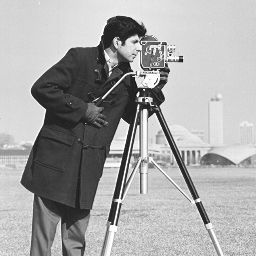
\includegraphics[scale=0.5]{imgs/cameraman.jpg}
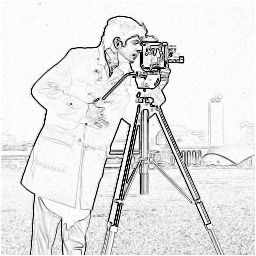
\includegraphics[scale=0.5]{imgs/cameraman-roberts-neg.jpg} \\*
\texttt{\small Ejemplo del filtro Roberts negado }\\
\end{center}

\pagebreak
%\vspace{10mm}
\subsection{Medición de Performance}

La siguiente tabla muestra la cantidad de ciclos mínima y promedio de cada implementación de los filtros, obtenidos de una muestra de
1000 ejecuciones de cada uno sobre la imagen de prueba \code{lena.bmp}:
\begin{center}
\begin{tabular}{|l|r|r|}
\hline
\multirow{2}{*}{Implementación}&\multicolumn{2}{|c|}{Ciclos de reloj} \\
\cline{2-3}
&Mínimo	&	Promedio \\
\hline
\multicolumn{3}{|c|}{Sobel}\\
\hline
Assembler	&	58.720.540	&	60.010.675 \\
\hline
C		&	393.586.848	&	416.838.429 \\
\hline
OpenCv		&	9.338.589	& 	9.797.886 \\
\hline
SSE		&	2.055.594 	&	2.078.737 \\
\hline
\multicolumn{3}{|c|}{Roberts}\\
\hline
Assembler	&	34.714.238	&	42.746.947 \\
\hline
C		&	320.676.453	&	336.808.912 \\
\hline
SSE		&	863.490		&	879.187 \\
\hline
\multicolumn{3}{|c|}{Prewitt}\\
\hline
Assembler	&	60.428.397	&	63.629.648 \\
\hline
C		&	634.337.521	&	664.132.063 \\
\hline
SSE		&	2.077.712	&	2.090.116 \\
\hline
\multicolumn{3}{|c|}{Frei-Chen}\\
\hline
SSE		&	4.005.108	&	4.038.886 \\
\hline
\end{tabular}
\end{center}

El rendimiento logrado con SSE es notable, las nuevas implementaciones son aproximadamente 30 veces más rápidas que las implementaciones sin SSE y en el 
caso de \keyword{Sobel}, es alrededor de 4 veces más rápida que la implementación original de la librería. Esto demuestra definitivamente el poder de 
trabajo de SSE para aplicaciones multimedia.

\pagebreak

